\section{Artículo principal}
\label{articulo_principal}

El artículo principal, \textit{A Note on ``Solving the Find-Path Problem by Good Representation of Free Space''}, es una crítica a un artículo de Brooks, llamado \textit{Solving the Find-Path Problem by Good Representation of Free Space}. En esta sección se llevará a cabo una introducción al artículo original de Brooks, explicando los puntos principales. Posteriormente, se explicarán las críticas que el artículo principal realiza sobre el artículo de Brooks.

\subsection{Solving the Find-Path Problem by Good Representation of Free Space}

El método que Brooks expone en este artículo se basa en la representación del espacio libre como conos generalizados. Un cono geralizado es un cono truncado que tiene una base y una tapa formada por cilindros (figura \ref{fig:cono_generalizado}).\\

\begin{figure}[h]
		\centering
        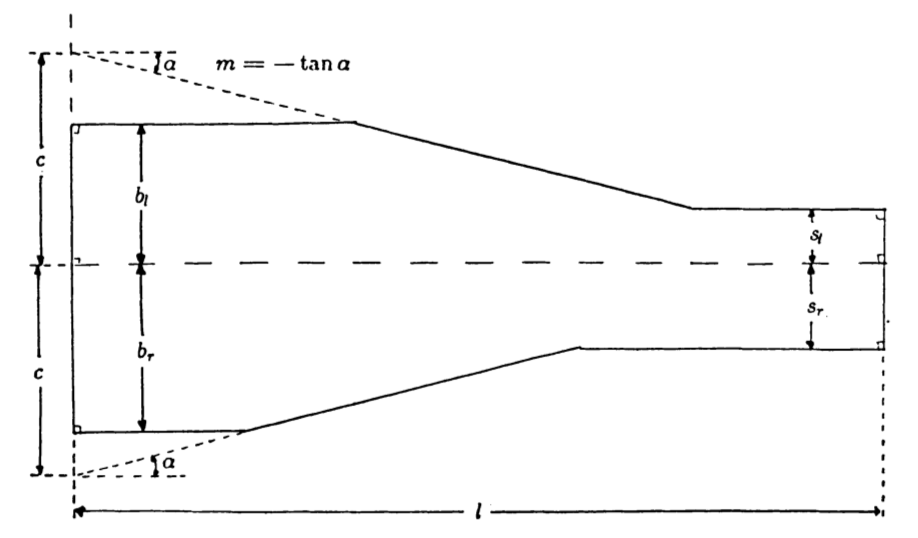
\includegraphics[width=0.5\textwidth]{images/cono_gen.png}
        \caption{Cono generalizado en un plano 2D}
        \label{fig:cono_generalizado}
\end{figure} 

El algoritmo propuesto es el siguiente. Primero, el mapa del entorno es analizado, y se calculan los conos generalizados que proporcionarán las trajectorias sin colisión. Este paso puede ser realizado en un tiempo $O(n^3)$. A continuación se procesan estos conos por parejas, comprobando para cuáles de ellos existe intersección entre sus columnas. La columna del cono generalizado es el eje de revolución del mismo. Hasta este punto, el algoritmo es independiente del objeto que se deseee mover por el entorno y, por tanto, sólo es necesario ejecutar esta parte del algoritmo una vez por cada entorno (suponiendo que el entorno es estático).\\

Cada intersección debe ser comprobada y anotada con el rango angular que describe las orientaciones del objeto en las que está garantizado que ese objeto quede contenido dentro del cono generalizado. De esta forma, se especifican las orientaciones o rotaciones permitidas para el objeto en cada una de las intersecciones.\\

Finalmente, se genera el grafo que contiene todas las rutas posibles, comprobando que, para cada intersección, el ángulo requerido para viajar de una intersección a la siguiente está contenido dentro del rango calculado en el paso anterior. Este grafo nos daría todas los caminos libres de colisión que existen en el entorno, asegurándonos que si viajamos desde un nodo A a un nodo B de este grafo con nuestro objeto no existirá colisión con ningún obstáculo. El hecho de usar las columnas de los conos generalizados nos grantiza también que el objeto recorrerá el camino lo más alejado posible de los obstáculos.\\

Una vez tenemos el grafo, se puede realizar la búsqueda del camino más corto de un nodo a otro del grafo usando un algoritmo de búsqueda en grafos tal como el $A^*$. El camino resultante será un conjunto de tramos rectos en los que el objeto se desplará usando translaciones puras y un conjunto de nodos en los que el objeto se reorientará mediante rotaciones puras para dirigirse al siguiente nodo.\\

El método para generar los conos generalizados está ampliamente detallado en el artículo, y se explica a continuación. En primer lugar, se define el lado libre de una arista del obstáculo como el lado hacia el que apunta la normal a esa superficie (la parte de fuera del polígono). Se considera que dos aristas forman parte de un cono generalizado si se cumplen las siguientes condiciones: al menos un vértice de la arista debe encontrarse en el lado libre de la otra arista y el producto escalar de las normales que apuntan hacia afuera debe ser negativo. Esta última condición asegura que los dos lados libres de las aristan se encuetren en el mismo lado.\\

Una vez se han calculado los conos generalizados, se obtienen las columnas de los mismos mediante la bisectriz del espacio libre entre las aristas de los obstáculos y se extiende el cono desde los vértices de forma paralela a su columna. Tras generar cada cono, se deben comprobar colisiones con todos los obstáculos, pues puede suceder que al generar un cono éste tenga un obstáculo dentro y no se encuentre totalmente en el espacio libre. Si esto sucede, la intersección se ha de proyectar sobre la columna del cono para obtener la parte del cono que pertece al espacio libre.\\

\subsection{A Note on ``Solving the Find-Path Problem by Good Representation of Free Space''}

Este artículo, escrito en 1997 por Wang, es una crítica al artículo de Brooks. En él, se explica que las condiciones de tranlaciones puras y rotaciones puras que son un requisito indispensable para la navegación usando el algoritmo de Brooks no son válidas para todos los tipos de robot móvil. Por tanto, el algoritmo de representación del espacio libre mediante conos generalizados sólo es aplicable a cierto tipo de robots móviles.\\

En primer lugar comenta las limitaciones en el caso de robots diferenciales, en cuyo caso las limitaciones sólo se aplican al punto de referencia que se ha de elegir para el sistema de referencia del robot. Para que las condiciones de rotación pura y translación puras se cumplan, el punto seleccionado debe encontrarse en el eje de rotación de las ruedas móviles, en el punto de corte con la mediatriz del eje.\\


En el caso de los robots de tres ruedas, tipo triciclo (figura \ref{fig:triciclo}) y los de cuatro, de tipo coche (con ruedas directrices y ruedas fijas), al ser robots no holonómicos,  además de la limitación del punto de referencia colocado en el punto medio del eje de las ruedas traseras, se añade una limitación extra para la rotación pura. De esta forma, si el robot posee un rango de movimiento en la rueda directriz menor de 90º, el robot no podrá realizar rotaciones puras. Esto se puede apreciar mediante las ecuaciones cinemáticas del robot de tipo triciclo:

\begin{figure}[h]
		\centering
        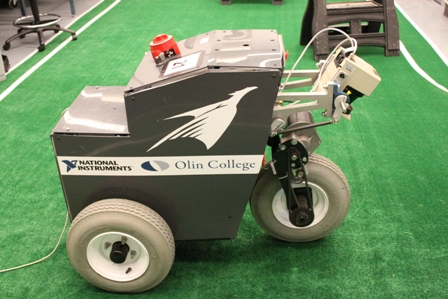
\includegraphics[width=0.5\textwidth]{images/triciclo.jpg}
        \caption{Robot tipo triciclo}
        \label{fig:triciclo}
\end{figure} 

\[ \dot{x_R} = - v \cos{(\alpha)} \sin{(\theta)} \]
\[ \dot{y_R} =   v \cos{(\alpha)} \cos{(\theta)} \]
\[ \dot{\theta} = \frac{v}{L} \sin{(\alpha)} \]\\

Para un punto situado en la rueda delantera, donde $\theta$ es el ángulo formado con la horizontal, $\alpha$ es el ángulo de giro de la rueda directriz, $v$ es la velocidad de la rueda directriz y L es la distancia entre el eje trasero y la rueda directriz. Para un punto situado en el punto medio del eje trasero, las ecuaciones cinemáticas se convierten en:

\[ \dot{x_R} = - v sin{(\alpha + \theta)} \]
\[ \dot{y_R} =   v \cos{(\alpha + \theta)} \]
\[ \dot{\theta} = \frac{v}{L} \sin{(\alpha)} \]\\

Con lo que podemos observar que sólo existe rotación pura para un robot de tipo triciclo si la rueda directriz no tiene limitado el rango de giro, y puede ir desde -90º hasta 90º. En todos los demás casos la rotación pura es imposible y, por tanto, no se podría aplicar el algoritmo de Brooks.


\newpage

